\documentclass{article}

\usepackage{xcolor}
\usepackage[final]{fri_rl_2026}
\usepackage[T1]{fontenc}
\renewcommand{\ttdefault}{lmtt}
\usepackage{microtype}
\usepackage{booktabs,array}
\usepackage{amsmath}
\usepackage{graphicx}

\title{When Should Noisy EEG Command a Simulated Robot?\\Continuous Gating and Irregular-Timing Request Control}

\author{
  Mario (\texttt{Mohnclizzy}) and Angel Lemus\\
  Department of Computer Science\\
  The University of Texas at Austin
}

\begin{document}
\maketitle

\begin{abstract}
When should noisy, nonstationary motor-imagery electroencephalography (EEG) command a stateful robotic manipulation skill? Offline window accuracy alone cannot answer this question: false activations move a robot during rest, whereas strict stabilization filters starve the controller during true imagery. We study this timing-versus-reliability tradeoff across two simulation studies combining project-built EEG decoders and supervisory command rules with an externally pretrained \texttt{robomimic} \texttt{BC-RNN} Franka lift policy wrapped in a project-built \texttt{HOLD} and completion-latch adapter (\texttt{robomimic-latch6-v2.0.0}).
In Study~1 (PhysioNet EEGBCI, 15 participants, 270 native MuJoCo rollouts), a selected moderate-hysteresis gate on \texttt{EEGNet8} transfer reduced \texttt{R08} development REST activation from 40.1\% to 27.9\% and imagery coverage from 52.1\% to 36.5\% (passing a predeclared utility screen in 7/15 participants). Across 270 matched robot rollouts, the gate lowered mean REST end-effector travel from 0.209\,m to 0.175\,m, yet retained 42/45 lifts versus 45/45 for raw commands (all three misses occurred in \texttt{S006}, whose gate enabled the robot for only 1.0\,s). Subsequent auditing revealed that PhysioNet \texttt{R04} and \texttt{R08} used identical cue schedules across all 15 participants (7,278/7,278 predictable endpoints without reading EEG), leaving the timing contribution of EEG unresolved.
We therefore ran Study~2 on recorded, acoustically cued EEG with irregular cue durations (1.50--8.36\,s imagery, 1.51--8.00\,s REST) from the four real human participants in BCI Competition~IV Dataset~1 (\texttt{ds1a}, \texttt{ds1b}, \texttt{ds1f}, \texttt{ds1g}; 720 held-out imagery episodes in reserved Runs~2--4), where clock-only baselines fell to 50.63\% and 50.01\% balanced accuracy. Under a single-request-starts-one-lift contract across 333 complete 20\,s slots and 240 versioned-harness rollouts (80 shared start offsets $\times$ 3 robot seeds; 0 post-acquisition drops), a frozen leaky evidence accumulator produced \textbf{154.0} imagery-triggered retained lifts (3-seed mean; 161 accepted starts), \textbf{59.0} REST-triggered lifts (62 starts), and \textbf{57.0} transition-triggered lifts (59 starts), compared with a single-frame EEG threshold (129.0 / 57.7 / 52.0 from 139 / 60 / 56 starts) and a matched-budget periodic timer (123.0 / 130.0 / 68.0 from 130 / 133 / 70 starts). On imagery-triggered retained lifts, the accumulator beat the periodic timer for 4/4 participants and the single-frame EEG threshold for 3/4 (on \texttt{ds1g}, the threshold produced 40.0 lifts versus 38.0 for the accumulator). Despite this timing gain, missed imagery remains the dominant failure mode: 465 of 720 imagery episodes (64.6\%) went undetected---including 105 of 115 short cues ($\le 2.5$\,s)---and 94 more (13.1\%) were blocked while the robot was busy or in the run tail.
\end{abstract}

%===============================================================================
\section{Introduction: From Offline Accuracy to When to Act}
\label{sec:intro}

Non-invasive EEG offers a low-cost assistive interface, yet motor-imagery recordings exhibit low signal-to-noise ratios, inter-subject variability, and strong nonstationarity~\citep{wolpaw2002,mcfarland2017,lotte2018}. While standard benchmarks emphasize fixed-epoch balanced accuracy~\citep{jayaram2018}, hierarchical shared autonomy~\citep{akinola2017} requires answering an operational question: \emph{when should noisy streaming probability estimates trigger or withhold a physical robot skill?} Continuous false activations during rest move the manipulator unintentionally, whereas over-conservative suppression delays or blocks legitimate requests~\citep{carrara2023}.

To isolate this command-timing question without conflating hardware failures with neural decoding error, we evaluate recorded public EEG replayed causally into a simulated robotic cube-lifting skill across two complementary studies. Table~\ref{tab:attribution} makes the system boundary explicit so every contribution is credited accurately: our team built the EEG preprocessing, decoders, supervisory command rules, timing/capacity audits, and simulation safety-latch harness, whereas public datasets supply neural recordings and an externally pretrained \texttt{robomimic} policy executes the low-level manipulation trajectory.

\begin{table}[h]
\centering
\caption{System boundary and explicit asset attribution across both simulation studies.}
\label{tab:attribution}
\footnotesize
\begin{tabular}{@{}p{0.27\linewidth}p{0.69\linewidth}@{}}
\toprule
\textbf{Component} & \textbf{Origin, role, and scope in this release} \\
\midrule
Public EEG datasets & \textbf{External.} Study~1: PhysioNet EEG Motor Movement/Imagery (\texttt{T0} rest vs.\ \texttt{T1}/\texttt{T2} left/right fist imagery, \texttt{S001}--\texttt{S015})~\citep{schalk2009}. Study~2: BCI Competition~IV Dataset~1 (\texttt{ds1a}, \texttt{ds1b}, \texttt{ds1f}, \texttt{ds1g}; 100\,Hz EEG + 1000\,Hz \texttt{true\_y})~\citep{blankertz2007,tangermann2012}. \\
Pretrained manipulation policy & \textbf{External.} \texttt{robomimic} Lift PH low-dimensional \texttt{BC-RNN} checkpoint (\texttt{lift\_ph\_low\_dim\_epoch\_1000\_\allowbreak succ\_100.pth}, SHA-256 \texttt{3ee222ca...})~\citep{mandlekar2021} in \texttt{robosuite~1.2} / \texttt{MuJoCo~2.1}~\citep{zhu2020robosuite,todorov2012mujoco}. Not trained by this project. \\
EEG preprocessing & \textbf{Project-built.} \texttt{MNE-Python}~\citep{gramfort2013} / SciPy common-average reference on 9 sensorimotor channels (\texttt{C3, Cz, C4, C1, C2, FC1, FC2, CP1, CP2}) and causal 4th-order 8--30\,Hz Butterworth \texttt{sosfilt} with 2.0\,s trailing windows at 4\,Hz. \\
EEG decoders & \textbf{Project-built.} Three decoder families: Common Spatial Patterns + Shrinkage LDA (\texttt{CSP/LDA})~\citep{blankertz2008}, OAS Riemannian Tangent Space + Shrinkage LDA (\texttt{Riemannian/LDA})~\citep{barachant2012}, and \texttt{EA-EEGNet8} transfer learning~\citep{lawhern2018}. \\
Command controllers \& \texttt{HOLD}/latch harness & \textbf{Project-built.} Continuous gates (raw, confidence, temporal, hysteresis, \texttt{q80}, \texttt{CRC}), discrete-request threshold and leaky accumulator, and versioned \texttt{robomimic-latch6-v2.0.0} \texttt{HOLD} + $+0.015$\,m $z$-latch wrapper. \\
\bottomrule
\end{tabular}
\end{table}

%===============================================================================
\section{Study 1: Continuous Gating on PhysioNet (15 Participants, 270 Rollouts)}
\label{sec:study1}

\subsection{Protocol, Decoder Selection, and Command Utility Screen}

In Study~1 (\texttt{results/\allowbreak bounded\_eeg\_robot\_2026-11-14/}), we evaluated 15 PhysioNet participants (\texttt{S001}--\texttt{S015}) under an exploratory development protocol that adapted decoders on run \texttt{R04} and compared gating rules on run \texttt{R08} (\texttt{R12} was excluded from this study). A preceding GPU transfer-learning campaign (\texttt{results/\allowbreak gpu\_campaign\_2026-11-13/}) spanning 54 complete recipe groups and 2,430 checkpoints identified full-transfer \texttt{EEGNet8} (\texttt{lr} $0.0001$, epoch 300; three seeds averaged within participant) as the top complete recipe by cue-window balanced accuracy at \textbf{68.15\%} (cohort SD 11.46\%), compared with \textbf{64.89\%} (SD 12.22\%) for \texttt{Riemannian/LDA} and \textbf{62.44\%} (SD 12.79\%) for \texttt{CSP/LDA}. Separately, an exploratory dense causal-window training ablation reported 62.52\% balanced accuracy, 42.07\% raw REST activation, and 40.61\% missed imagery; however, a subsequent engineering audit (documented in \texttt{results/\allowbreak project\_review\_2026-11-18/\allowbreak review.md}) established that the dense run executed 178 source updates per epoch versus 42 in the original recipe, so it cannot isolate windowing effects under matched optimization budgets.

\begin{figure}[t]
\centering
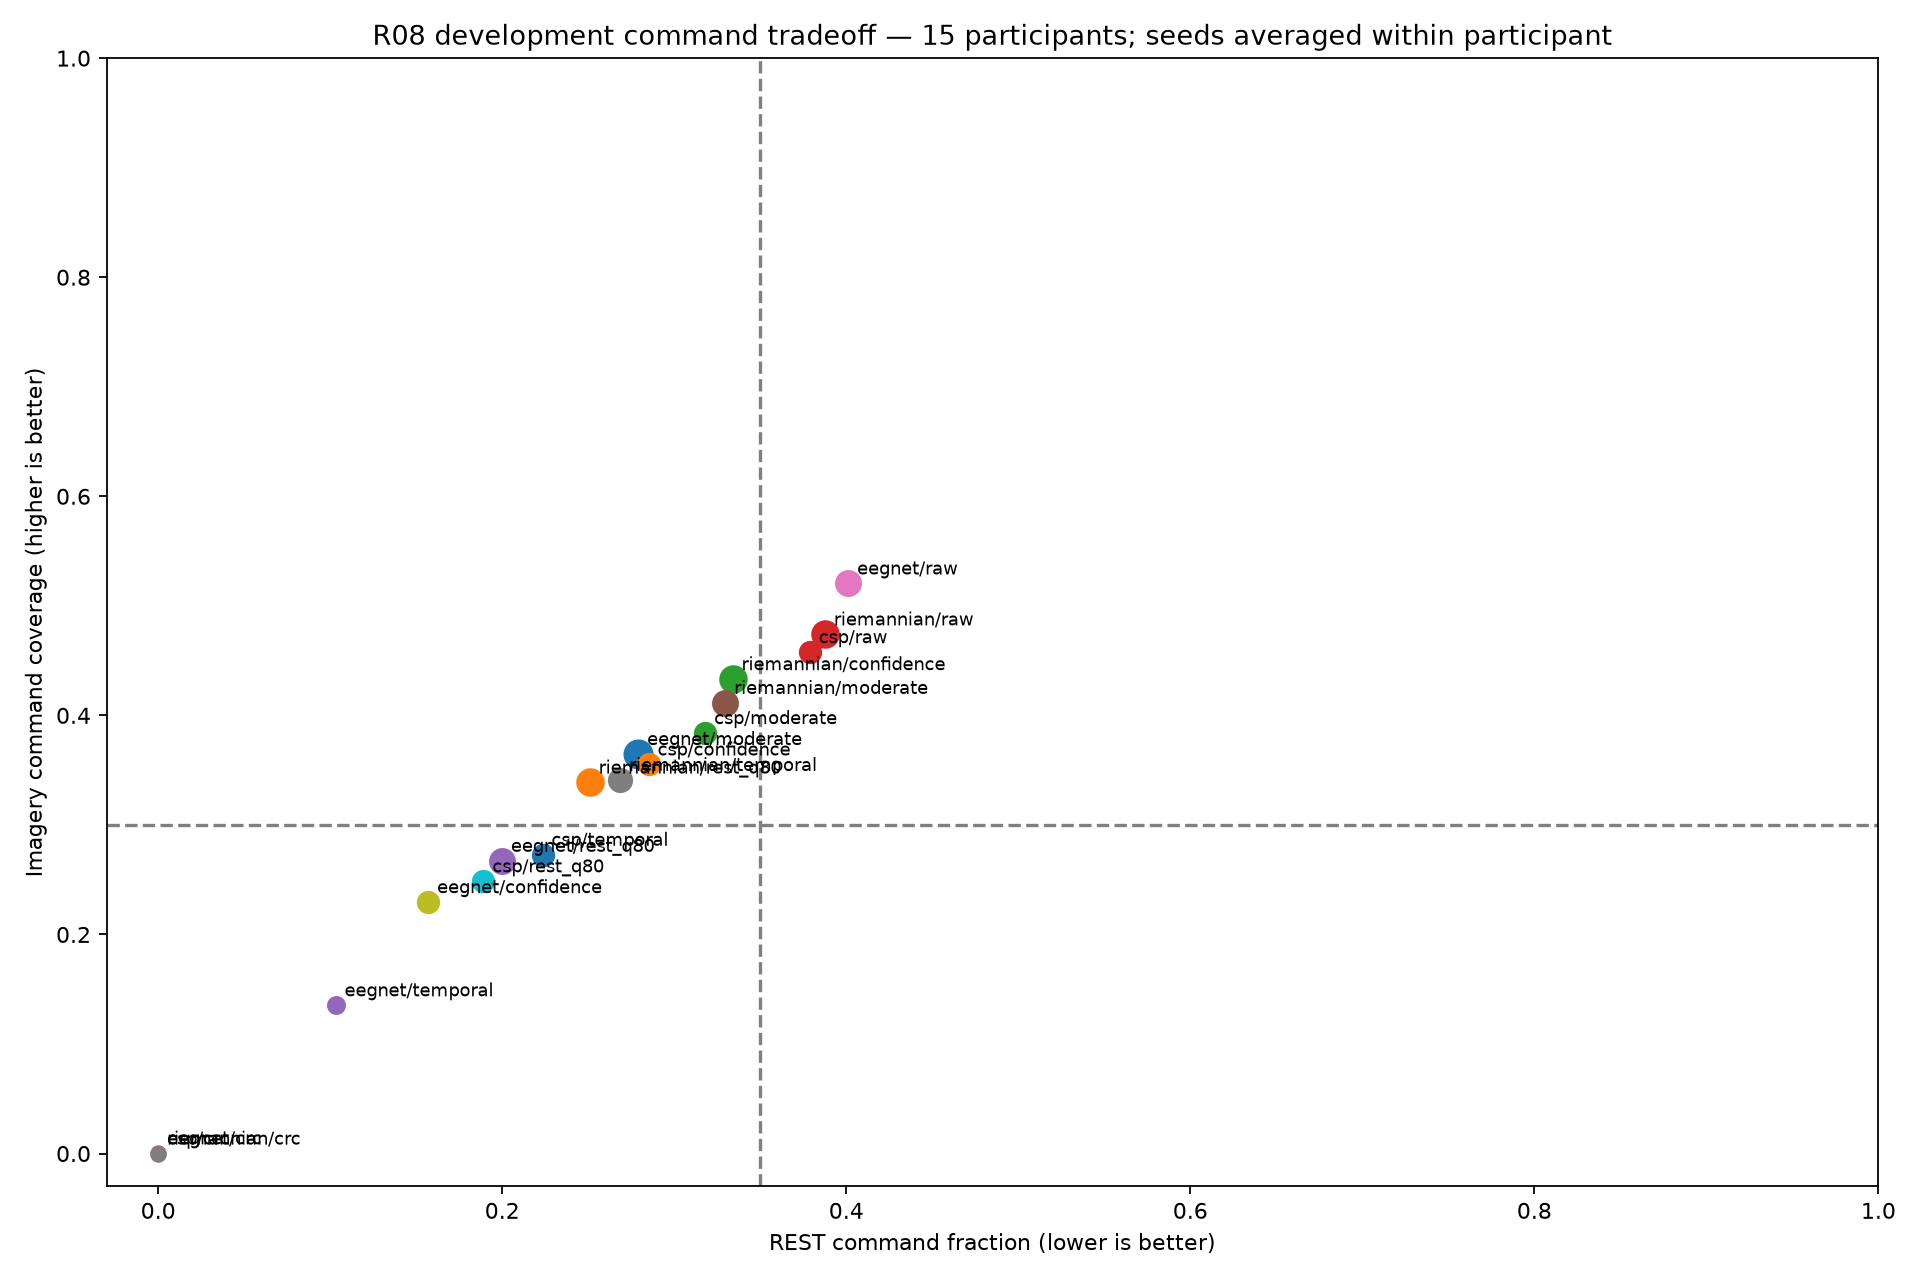
\includegraphics[width=0.92\textwidth]{../../results/bounded_eeg_robot_2026-11-14/command_tradeoff.png}
\caption{\textbf{Study 1 continuous-gating tradeoff on PhysioNet \texttt{R08} ($N=15$ participants; three \texttt{EEGNet} seeds averaged per participant).} Dashed reference lines mark the predeclared utility thresholds ($\le 35\%$ REST command fraction, $\ge 30\%$ imagery command coverage). The selected \texttt{eegnet/moderate} hysteresis gate reduces mean REST activation from 40.1\% (\texttt{eegnet/raw}) to 27.9\% while lowering imagery coverage from 52.1\% to 36.5\%, passing the utility screen for 7/15 participants (vs.\ 5/15 for raw and 0/15 for conformal risk control \texttt{CRC}). Figure reused from \texttt{results/\allowbreak bounded\_eeg\_robot\_2026-11-14/\allowbreak command\_tradeoff.png}.}
\label{fig:study1_tradeoff}
\end{figure}

Sweeping six candidate gates across all three decoder families on \texttt{R08} (Figure~\ref{fig:study1_tradeoff}) showed that calibration-strict Conformal Risk Control (\texttt{CRC}) emitted nearly 0 commands across all decoders (0/15 passing). The strongest candidate under our predeclared utility screen (\texttt{eegnet/moderate}, threshold $0.55$, hysteresis margin $0.02$, persistence $0.25$\,s) reduced mean REST activation from \textbf{40.1\%} (\texttt{eegnet/raw}) to \textbf{27.9\%}, at the cost of lowering imagery coverage from \textbf{52.1\%} to \textbf{36.5\%}, and passed for 7/15 participants (compared with 5/15 for \texttt{eegnet/raw} and 6/15 for top \texttt{Riemannian} gates).

\subsection{270-Rollout Continuous Robot Tradeoff}

To measure how continuous gating affects physical execution, we replayed causal 20\,s (400-step at 20\,Hz) \texttt{R08} decision streams across all 15 participants $\times$ 3 shared simulated robot starting states (\texttt{seeds 0, 1, 2}) $\times$ 6 conditions (\textbf{270 native rollouts} total) under \texttt{robomimic-latch6-v2.0.0}. Once the policy acquires bilateral gripper contact for 10 consecutive steps at $\ge 0.08$\,m cube rise, a non-learned completion latch applies a one-time $+0.015$\,m $z$-offset and freezes the end-effector goal through step 400. Note that seeds represent simulator initial-state variance across three shared starts rather than 45 independent participants.

\begin{table}[t]
\centering
\caption{\textbf{Study 1 robot outcomes across 270 native MuJoCo rollouts (PhysioNet \texttt{R08}, 45 rollouts/condition = 15 participants $\times$ 3 shared robot seeds, 20\,s horizon).} Group means use exact values from \texttt{results/\allowbreak bounded\_eeg\_robot\_2026-11-14/\allowbreak robot/\allowbreak robot\_results/\allowbreak aggregate.json}.}
\label{tab:study1_robot}
\resizebox{\textwidth}{!}{%
\footnotesize
\setlength{\tabcolsep}{4.0pt}
\begin{tabular}{@{}lrrrrrrrr@{}}
\toprule
\textbf{Condition} & \textbf{Retained} & \textbf{Acq.\ step} & \textbf{Req.\ enable} & \textbf{Policy calls} & \textbf{Latch} & \textbf{Req.\ REST} & \textbf{REST EEF} & \textbf{REST moving} \\
 & & \textbf{(20\,Hz)} & \textbf{(s / 20\,s)} & \textbf{(s)} & \textbf{(s)} & \textbf{enable (\%)} & \textbf{path (m)} & \textbf{time (s)} \\
\midrule
\textbf{Selected EEGNet gate} & \textbf{42 / 45} & 153.4 & 9.32 & 2.22 & 11.51 & 38.9\% & \textbf{0.175} & 1.94 \\
Raw EEGNet commands & \textbf{45 / 45} & 139.3 & 11.83 & 2.29 & 13.03 & 51.0\% & \textbf{0.209} & 2.04 \\
Always-enable & 45 / 45 & 53.0 & 20.00 & 2.65 & 17.35 & 100.0\% & 0.387 & 3.37 \\
Always-HOLD & 0 / 45 & --- & 0.00 & 0.00 & 0.00 & 0.0\% & 0.029 & 0.58 \\
Duration-matched contiguous & 42 / 45 & 53.0 & 9.32 & 2.54 & 16.19 & 50.7\% & 0.374 & 3.25 \\
Selected shifted $+10$\,s & 40 / 45 & 125.4 & 9.32 & 2.42 & 12.82 & 42.5\% & 0.266 & 2.68 \\
\bottomrule
\end{tabular}%
}
\end{table}

Table~\ref{tab:study1_robot} summarizes the physical tradeoff. Compared with \texttt{raw}, the \texttt{selected} gate reduced requested enable time during annotated REST from 51.0\% to 38.9\% (4.59\,s of the 11.8\,s REST window) and lowered mean REST end-effector path from \textbf{0.209\,m} to \textbf{0.175\,m} (paired difference $-0.034$\,m, negative for 10/15 participants; an unresolved point estimate at $N=15$). Actual executed policy calls differed little (2.22\,s vs.\ 2.29\,s) because the completion latch already halts policy execution after lift acquisition. Meanwhile, retention dropped from \textbf{45/45} to \textbf{42/45}: all three misses belonged to one participant (\texttt{S006}), whose selected gate delivered only 20 enabled steps (1.0\,s), insufficient for the policy to reach the cube (duration-matched \texttt{contiguous} also retained 42/45, failing on \texttt{S006}). A representative rollout video from Study~1 is committed at \texttt{results/\allowbreak bounded\_eeg\_robot\_2026-11-14/\allowbreak robot/\allowbreak robot\_results/\allowbreak S001\_seed0\_selected/\allowbreak video.mp4} and shows \textbf{PhysioNet \texttt{R08}, participant \texttt{S001}, robot \texttt{seed~0}, \texttt{selected} \texttt{eegnet/moderate} condition} (\texttt{complete\_retained}, acquisition at step 137 / 6.85\,s, 52 executed policy calls, 0.096\,m terminal rise; selected by fixed participant/seed order).

\subsection{Why Predictable PhysioNet Cues Motivated an Irregular-Timing Test}

Our November~18 engineering audit (\texttt{results/project\_review\_2026-11-18/review.md}, verified by \texttt{analysis/audit\_cue\_clock.py} and \texttt{analysis/request\_capacity.py}) uncovered two structural constraints in PhysioNet:
\begin{enumerate}
  \item \textbf{Identical cue schedules across runs:} Across all 15 participants, \texttt{R04} and \texttt{R08} have identical binary cue interval lists. Replaying each person's \texttt{R04} cue schedule against the \texttt{R08} recording clock predicted \textbf{7,278 / 7,278 (100\%)} annotated 4\,Hz \texttt{R08} endpoints without reading EEG at all, and even a fixed 4.1\,s periodic timer achieved 96.08\% balanced accuracy.
  \item \textbf{20\,s robot-slot capacity ceiling:} Under a nonoverlapping 20\,s single-request scheduler (one lift per 20\,s slot), \texttt{R08} contains 90 complete 20\,s slots versus 225 instructed imagery episodes (222 overlapping the robot horizon), creating an annotation-only ceiling of \textbf{40.0\%} (90/225; 40.6\% per-participant robot-horizon mean). Stream request detection must therefore be scored separately from robot slot acceptance.
\end{enumerate}

\section{Study 2: Request Timing Under Variable Cues (BCI Competition~IV Dataset~1)}
\label{sec:study2}

\subsection{Dataset Audit, Causality, and One-Request Robot Contract}

To test whether EEG adds timing value when a clock fails, we evaluated BCI Competition~IV Dataset~1 (\texttt{results/bciciv\_ds1\_request\_pilot\_2026-11-19/}) using the official 100\,Hz EEG archive (\texttt{BCICIV\_1\_mat.zip}) and 1000\,Hz ground-truth evaluation labels (\texttt{true\_labels.zip}). Following dataset documentation, we retained the four real human participants (\texttt{ds1a}, \texttt{ds1b}, \texttt{ds1f}, \texttt{ds1g}) and excluded the three artificially generated datasets (\texttt{ds1c}, \texttt{ds1d}, \texttt{ds1e}; our clock audit \texttt{analysis/audit\_bciciv\_ds1\_clock.py} also detected that artificial \texttt{ds1c} duplicated Run~1 exactly in Run~3, scoring 1.0000). Across the four human recordings (verified 10:1 sample alignment through the full tail of \texttt{ds1a} Run~4), spoken start and stop cues occurred at unpredictable intervals: full imagery cues lasted \textbf{1.50--8.36\,s} (960 episodes total) and full REST cues lasted \textbf{1.51--8.00\,s} (944 episodes). When scored at 4\,Hz (\texttt{report/final/bciciv\_ds1\_clock\_audit.json}), replaying Run~1's continuous cue schedule on Runs~2--4 dropped to \textbf{50.63\%} mean balanced accuracy (51.44\%, 47.65\%, 49.87\%, 53.57\%) and the fixed 4.1\,s timer dropped to \textbf{50.01\%}.

This second experiment evaluates \emph{recorded, acoustically cued imagery and simulated execution}, not self-paced voluntary control. For each human participant (\texttt{analysis/bciciv\_ds1\_request\_pilot.py}), we fitted a 3-class \texttt{OAS Riemannian Tangent Space + Shrinkage LDA} decoder on the 9 central channels using \textbf{Evaluation Run~1} only (causal 8--30\,Hz \texttt{sosfilt}, 2.0\,s trailing windows at 4\,Hz; $p_{\text{MI}} = 1 - p_{\text{REST}}$). Using 5-fold chronological out-of-fold probabilities on Run~1 (with $\pm 2.0$\,s fold boundary guards), we selected thresholds under a shared development budget of $\le 3.0$ false starts per REST minute for three frozen controllers: (1) a \textbf{periodic timer} ($T \in [15.0, 19.0]$\,s), (2) a \textbf{single-frame EEG threshold} ($p_{\text{MI}} \ge \theta$, $\theta \in [0.79, 0.91]$, with 0.5\,s $< 0.5$ re-arm and 1.0\,s refractory period), and (3) an \textbf{EEG sustained leaky accumulator} updated while armed as $A_t = \max(0,\, e^{-\Delta t / \tau_{\text{decay}}} A_{t-1} + \Delta t\, e_t)$ with decay constant $\tau_{\text{decay}} = 1.0$\,s, elapsed step $\Delta t$ ($0.25$\,s at 4\,Hz), clipped evidence $e_t = \operatorname{clip}(\operatorname{logit}(\tilde{p}_{\text{MI},t}) - \operatorname{logit}(0.55), -2, 2)$ relative to fixed baseline $p_0 = 0.55$ ($\tilde{p}_{\text{MI},t} \in [10^{-6}, 1-10^{-6}]$), trigger threshold $A_{\text{th}} \in [0.50, 1.05]$, and post-request reset $A_t \leftarrow 0$ under the same 0.5\,s $< 0.5$ re-arm and 1.0\,s refractory rules (holding $A_t = 0$ while disarmed). All parameters were frozen and run continuously across reserved \textbf{Evaluation Runs~2--4} (180 imagery episodes per person = \textbf{720 total}; 333 complete nonoverlapping 20\,s slots = 83+85+82+83). Official 1.0\,s post-cue \texttt{NaN} transition masks were applied \emph{only at scoring}.

Under the discrete one-request-starts-one-lift robot contract (\texttt{simulation/\allowbreak scripts/\allowbreak run\_one\_\allowbreak request\_\allowbreak window\_\allowbreak grid.py}), the first emitted request inside an idle 20\,s slot triggers a 400-step \texttt{robomimic-latch6-v2.0.0} rollout starting at 20\,Hz step $s_{\text{start}} = \operatorname{round}(t_{\text{rel}} \cdot 20) + 1 \in \{1, 6, \dots, 396\}$ across three shared robot seeds (\texttt{0, 1, 2}); subsequent requests in that slot are rejected as busy. Across all \textbf{240 native rollouts} (80 start offsets $\times$ 3 seeds, shared across participants), 100\% passed all \texttt{HOLD}, latch, and contact-proxy invariants with \textbf{0 post-acquisition drops} (\texttt{post\_acquisition\_loss = False} in 240/240). Every robot outcome is labeled by instructed human state \textbf{at request time}, and retained-lift totals are \textbf{3-seed means} over the shared robot seeds.

\begin{figure}[t]
\centering
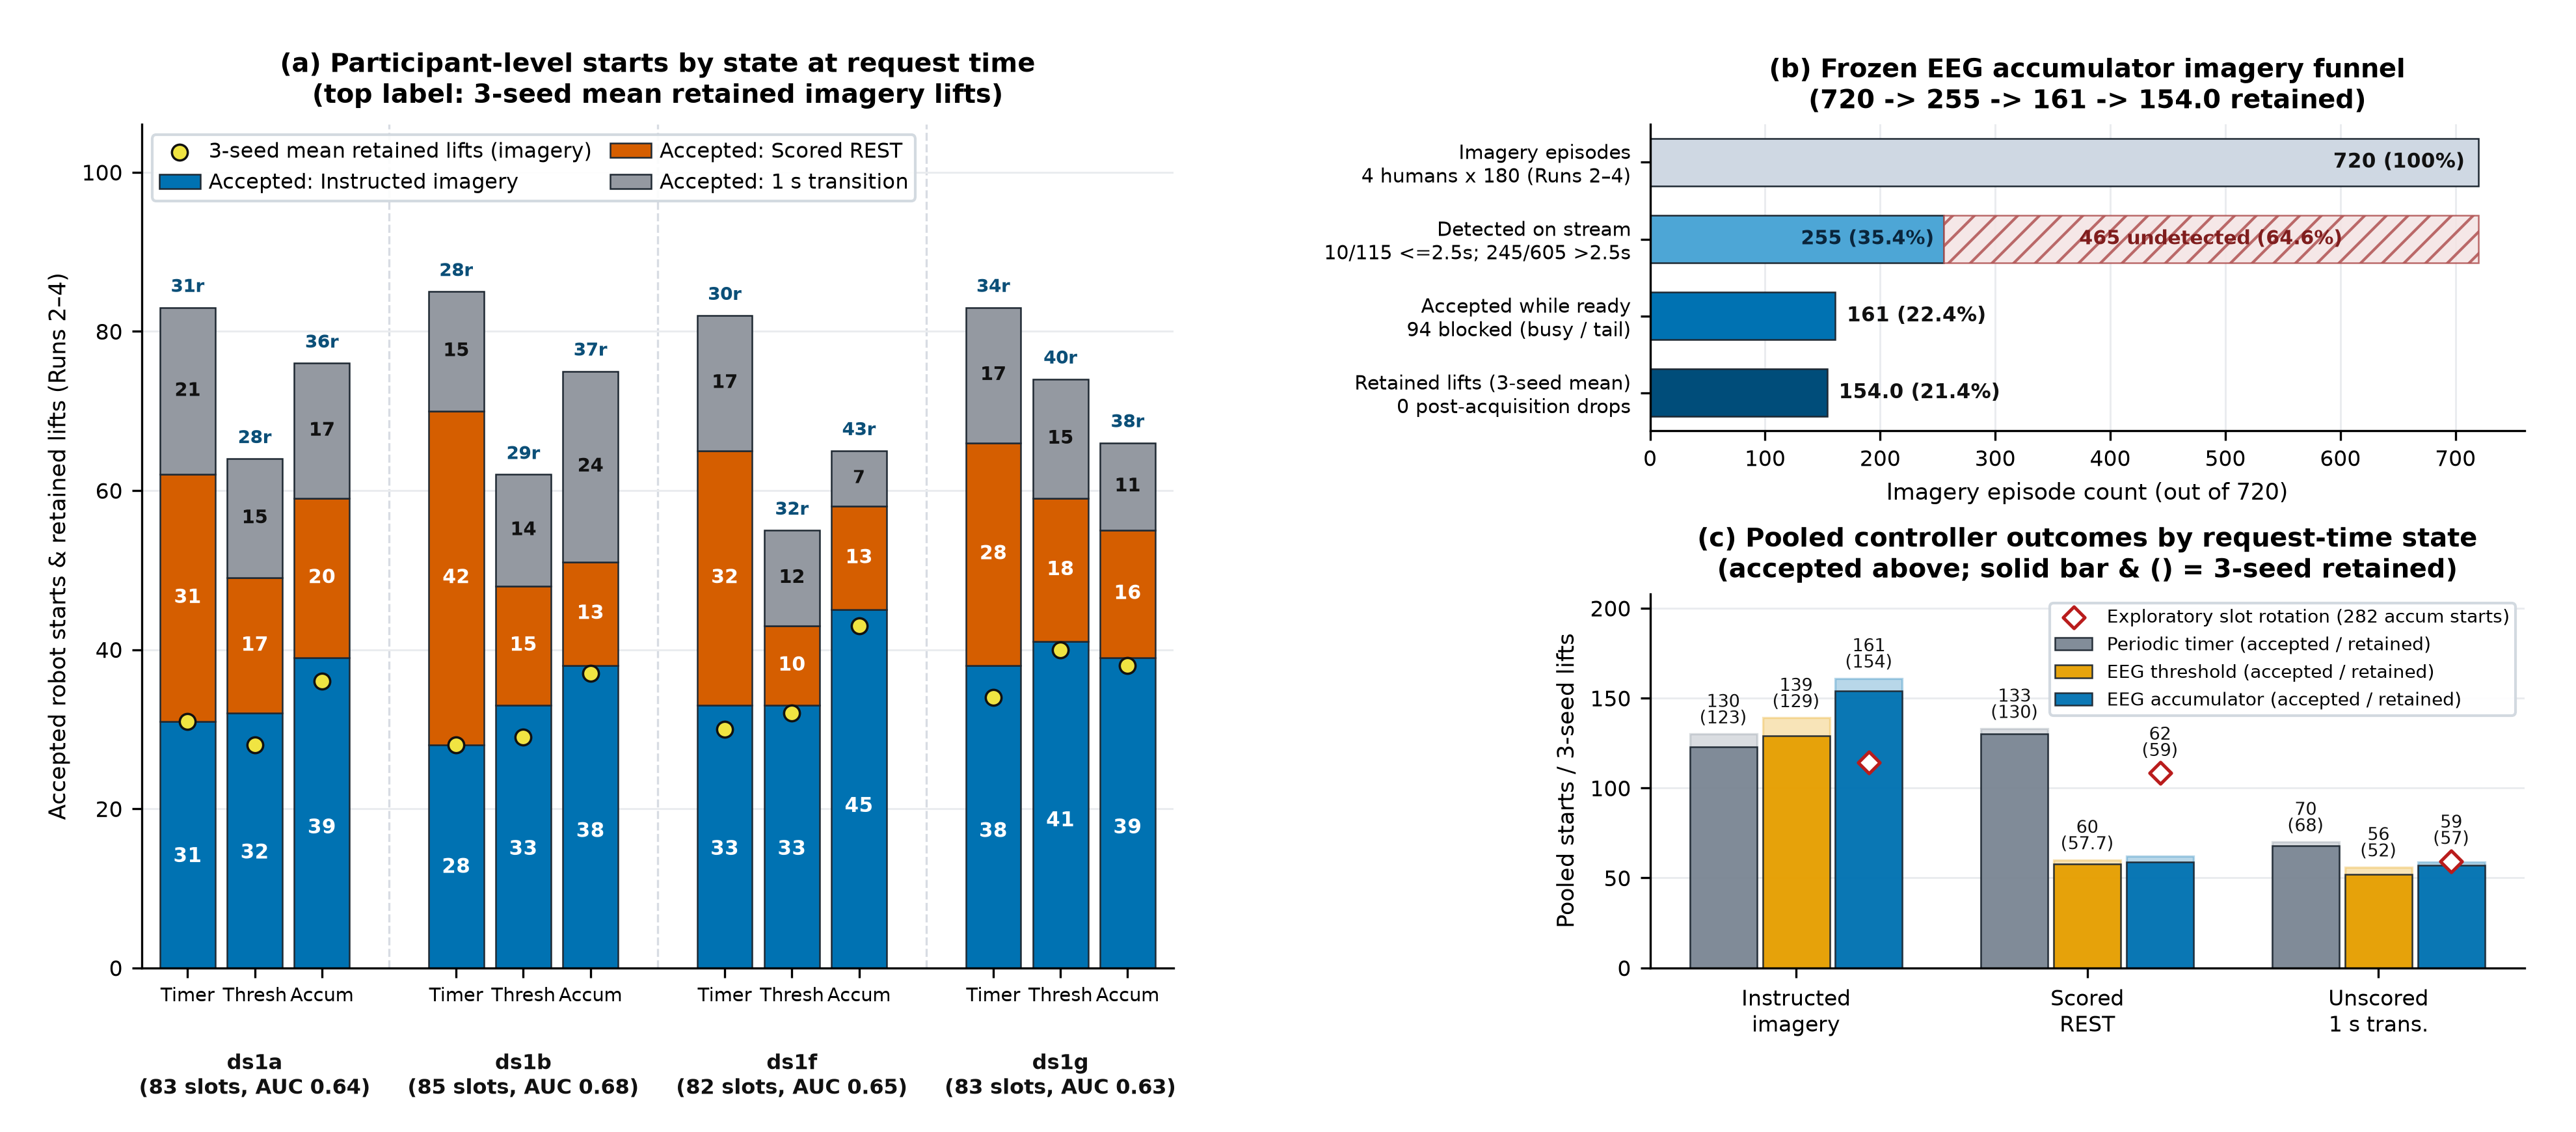
\includegraphics[width=\textwidth]{figures/bciciv_ds1_pilot_overview.png}
\caption{\textbf{Study 2 irregular-timing request pilot on BCI Competition~IV Dataset~1 (reserved Runs~2--4 across four human participants, 720 imagery episodes, 333 complete 20\,s slots, 240 native rollouts).} \textbf{(a)} Accepted robot starts stacked by instructed state at request time for all four humans and all three controllers, with yellow circles and top labels reporting 3-seed mean continuously retained imagery lifts. \textbf{(b)} Frozen EEG accumulator attrition from 720 imagery episodes to 255 stream detections (465 undetected, including 105/115 short cues $\le 2.5$\,s), 161 accepted starts (94 blocked by busy slots/tail), and \textbf{154.0} retained lifts (3-seed mean, 0 drops). \textbf{(c)} Pooled accepted starts and 3-seed retained lifts by request-time state, alongside the \emph{exploratory} circular slot-rotation timing control (red diamonds) on the 282 accepted accumulator starts.}
\label{fig:study2_overview}
\end{figure}

\subsection{Pooled Comparison: Emitted vs.\ Accepted vs.\ Continuously Retained Lifts}

Table~\ref{tab:study2_pooled} and Figure~\ref{fig:study2_overview} separate pre-scheduler stream emissions (Runs~2--4), scheduler acceptance (333 complete 20\,s slots), and continuous lift retention (3-seed means). Accumulating causal evidence produced \textbf{154.0} continuously retained lifts triggered during instructed imagery (161 accepted starts; 7.18\,s mean within-slot request time, 2.01\,s mean stream onset delay across detected episodes) while limiting REST-triggered retained lifts to \textbf{59.0} (62 starts) and unscored transition lifts to \textbf{57.0} (59 starts: 27 in the 1\,s post-start-cue window, 32 in the 1\,s post-stop-cue window, with only 2/32 crossing a 20\,s slot boundary). Relative to the periodic timer (\textbf{123.0} imagery / \textbf{130.0} REST retained lifts), the accumulator delivered $+31.0$ imagery lifts and $-71.0$ unwanted REST lifts. Relative to the single-frame EEG threshold (\textbf{129.0} imagery / \textbf{57.7} REST retained lifts), accumulating evidence added $+25.0$ imagery lifts for only $+1.3$ REST lifts.

As an \textbf{exploratory timing control}, we preserved all 282 accepted accumulator starts and their exact within-slot offsets while circularly rotating slots (non-zero shifts) within each recording (\texttt{pilot\_metrics.json}). Rotated slots averaged \textbf{114.3} imagery, \textbf{108.3} REST, and \textbf{59.4} transition starts versus the observed \textbf{161}, \textbf{62}, and \textbf{59}, supporting that the gain reflects temporal alignment to instructed imagery rather than merely triggering less often than the timer (282 vs.\ 333 starts).

\begin{table}[t]
\centering
\caption{\textbf{Study 2 pooled Runs~2--4 results across all four real human participants (720 imagery episodes, 333 complete 20\,s slots, 240 versioned native rollouts).} Robot outcomes are labeled by instructed state \emph{at request time}; lift counts are 3-seed means over shared starts (\texttt{0} post-acquisition drops).}
\label{tab:study2_pooled}
\footnotesize
\setlength{\tabcolsep}{5.0pt}
\begin{tabular}{@{}lrrr@{}}
\toprule
\textbf{Stage \& metric} & \textbf{Periodic timer} & \textbf{EEG threshold} & \textbf{EEG accumulator} \\
\midrule
\multicolumn{4}{@{}l}{\emph{Full-stream emissions (pre-scheduler, Runs 2--4)}} \\
Emitted requests total & 401 & 384 & 469 \\
--- First imagery detections (+ duplicates) & 149 (+0) & 211 (+4) & 255 (+7) \\
--- Undetected imagery episodes (out of 720) & 571 & 509 & 465 \\
--- Emitted during scored REST & 168 & 89 & 116 \\
--- Emitted during unscored 1\,s transitions & 84 & 80 & 91 \\
\midrule
\multicolumn{4}{@{}l}{\emph{Robot scheduler acceptance (333 complete 20\,s slots)}} \\
Accepted robot starts total & \textbf{333} & \textbf{255} & \textbf{282} \\
--- During instructed imagery & \textbf{130} & \textbf{139} & \textbf{161} \\
--- During scored REST & \textbf{133} & \textbf{60} & \textbf{62} \\
--- During unscored transitions (start / stop) & 70 (39 / 31) & 56 (28 / 28) & 59 (27 / 32) \\
Rejected busy (+ incomplete tail) & 59 (+9) & 123 (+6) & 178 (+9) \\
\midrule
\multicolumn{4}{@{}l}{\emph{Verified continuous retention (robomimic-latch6-v2.0.0, 3-seed mean)}} \\
Total continuously retained lifts & 321.0 & 238.7 & 270.0 \\
--- \textbf{Started during instructed imagery} & \textbf{123.0} & \textbf{129.0} & \textbf{154.0} \\
--- \textbf{Started during scored REST} & \textbf{130.0} & \textbf{57.7} & \textbf{59.0} \\
--- Started during unscored 1\,s transitions & 68.0 & 52.0 & 57.0 \\
Post-acquisition drops (across all 240 rollouts) & 0 & 0 & 0 \\
\bottomrule
\end{tabular}
\end{table}

\subsection{Individual Differences Across Participants and Missed-Cue Attrition}

Table~\ref{tab:study2_participants} reports all four human participants individually. Runs~2--4 window ROC-AUC ranged modestly from 0.631 (\texttt{ds1g}) to 0.680 (\texttt{ds1b}). Under the frozen Run~1 threshold budget ($\le 3.0$\,FS/REST-min), all four participants achieved more imagery starts and fewer REST starts with the EEG accumulator than with the periodic timer (4/4 participant consistency). However, individual dynamics diverged notably: on \texttt{ds1a}, out-of-budget drift pushed the frozen accumulator to 3.29\,FS/REST-min (38 REST starts) vs.\ 2.25 for the EEG threshold; on \texttt{ds1f}, the accumulator gained $+12$ accepted imagery starts over both baselines with only 13 REST starts; and on \texttt{ds1g}, the simpler single-frame EEG threshold slightly outperformed the accumulator on imagery detections (63 vs.\ 55) and retained imagery lifts (40.0 vs.\ 38.0) at nearly identical REST starts (18 vs.\ 16).

Crucially, Figure~\ref{fig:study2_overview}(b) shows that \textbf{missing intended cues remains the main bottleneck}: across 720 imagery episodes, the accumulator never emitted a request inside \textbf{465 episodes (64.6\%)}, emitted 94 valid detections (13.1\%) while the robot was already busy in its 20\,s slot (or in the unscheduled run tail), and converted 161 episodes (22.4\%) into accepted starts (\textbf{154.0} retained lifts). Short cues ($\le 2.5$\,s full cue duration, $\le 1.5$\,s unmasked; 115 episodes) were especially hard: the accumulator detected only \textbf{10 / 115 (8.7\%)} short episodes compared with \textbf{245 / 605 (40.5\%)} longer episodes ($> 2.5$\,s).

\begin{table}[t]
\centering
\caption{\textbf{Study 2 per-participant breakdown on reserved Runs~2--4 (180 imagery episodes per participant).} Reported metrics trace directly to \texttt{results/\allowbreak bciciv\_ds1\_request\_pilot\_2026-11-19/\allowbreak pilot\_metrics.json}.}
\label{tab:study2_participants}
\resizebox{\textwidth}{!}{%
\footnotesize
\setlength{\tabcolsep}{3.8pt}
\begin{tabular}{@{}lrrrrrr@{}}
\toprule
\textbf{Part.\ (Slots, AUC)} & \textbf{Controller} & \textbf{Stream Det.} & \textbf{FS/min} & \textbf{Acc.\ Img /} & \textbf{Busy Rej.} & \textbf{Ret.\ Lifts (3-seed)} \\
 & & \textbf{(out of 180)} & \textbf{(REST)} & \textbf{REST / Trans} & \textbf{(+Tail)} & \textbf{Img / REST / Trans} \\
\midrule
\texttt{ds1a} (83, 0.644) & Periodic timer ($15.0$\,s) & 40 (22.2\%) & 3.99 & 31 / 31 / 21 & 28 (+4) & 31.0 / 31.0 / 21.0 \\
 & EEG threshold ($0.91$) & 48 (26.7\%) & 2.25 & 32 / 17 / 15 & 27 (+4) & 28.0 / 17.0 / 15.0 \\
 & EEG accumulator ($1.05$) & \textbf{68 (37.8\%)} & 3.29 & \textbf{39} / 20 / 17 & 50 (+6) & \textbf{36.0} / 19.0 / 16.0 \\
\midrule
\texttt{ds1b} (85, 0.680) & Periodic timer ($16.5$\,s) & 34 (18.9\%) & 4.79 & 28 / 42 / 15 & 19 (+2) & 28.0 / 42.0 / 15.0 \\
 & EEG threshold ($0.91$) & 51 (28.3\%) & 1.45 & 33 / 15 / 14 & 25 (+0) & 29.0 / 13.0 / 14.0 \\
 & EEG accumulator ($0.97$) & \textbf{69 (38.3\%)} & 1.90 & \textbf{38} / 13 / 24 & 53 (+0) & \textbf{37.0} / 11.0 / 23.0 \\
\midrule
\texttt{ds1f} (82, 0.652) & Periodic timer ($19.0$\,s) & 35 (19.4\%) & 3.16 & 33 / 32 / 17 & 6 (+2) & 30.0 / 30.0 / 16.0 \\
 & EEG threshold ($0.79$) & 49 (27.2\%) & 1.32 & 33 / 10 / 12 & 27 (+2) & 32.0 / 10.0 / 9.0 \\
 & EEG accumulator ($0.50$) & \textbf{63 (35.0\%)} & 2.29 & \textbf{45} / 13 / 7 & 40 (+3) & \textbf{43.0} / 13.0 / 7.0 \\
\midrule
\texttt{ds1g} (83, 0.631) & Periodic timer ($18.75$\,s) & 40 (22.2\%) & 3.18 & 38 / 28 / 17 & 6 (+1) & 34.0 / 27.0 / 16.0 \\
 & EEG threshold ($0.82$) & \textbf{63 (35.0\%)} & 3.08 & \textbf{41} / 18 / 15 & 44 (+0) & \textbf{40.0} / 17.7 / 14.0 \\
 & EEG accumulator ($0.97$) & 55 (30.6\%) & 2.98 & 39 / 16 / 11 & 35 (+0) & 38.0 / 16.0 / 11.0 \\
\bottomrule
\end{tabular}%
}
\end{table}

%===============================================================================
\section{Limitations, Reproducibility, and Scoped Follow-Up}
\label{sec:limits}

Several boundaries constrain interpretation across both studies:
(1) \textbf{Cued replay vs.\ self-paced BCI:} Both datasets use externally paced visual or spoken cues replayed causally offline; our results establish request timing relative to instructed states, not online closed-loop adaptation, voluntary un-cued intent, or physical safety on real hardware.
(2) \textbf{Cohort size and selection bias:} Study~1 (\texttt{N=15}) selected gates directly on \texttt{R08} and suffered from predictable cues; Study~2 (\texttt{N=4} real humans) isolates genuine irregular-timing signal value within four people but cannot estimate population-level clinical reliability.
(3) \textbf{Shared simulated starts:} In both robot batches, seeds \texttt{0, 1, 2} parameterize simulator variability across shared initial cube poses rather than independent human trials.
(4) \textbf{Unresolved short-cue delay vs.\ unequal observation time:} Only 10/115 short imagery cues ($\le 2.5$\,s) triggered the accumulator. Longer episodes inherently afford more time after the 2.0\,s decoder window and 1.0\,s scoring mask; whether short cues are intrinsically harder at matched elapsed time remains an open empirical question scoped separately in Milestones~5--6 of \texttt{docs/\allowbreak ANTIGRAVITY\_ROADMAP.md}.

Complete CPU reproduction instructions---covering the \textbf{short route} (verifying committed manifests and rebuilding figures/tables via \texttt{analysis/\allowbreak build\_final\_report\_artifacts.py}) and the \textbf{full route} (downloading official \texttt{bbci.de} archives, running \texttt{analysis/\allowbreak audit\_bciciv\_ds1\_clock.py} and \texttt{analysis/\allowbreak bciciv\_ds1\_request\_pilot.py}, and documenting Linux/WSL2 regeneration of the 240 native MuJoCo rollouts via \texttt{simulation/\allowbreak scripts/\allowbreak run\_one\_request\_window\_grid.py})---are documented in \texttt{docs/\allowbreak REPRODUCTION\_GUIDE.md}.

\acknowledgments{We thank Schalk et al.\ for the PhysioNet EEG Motor Movement/Imagery Dataset, Blankertz et al.\ and the Berlin BCI group for BCI Competition~IV Dataset~1, Mandlekar et al.\ for the pretrained \texttt{robomimic} Lift \texttt{BC-RNN} policy, the developers of \texttt{MNE-Python}, \texttt{robosuite}, and \texttt{MuJoCo}, and the Freshman Research Initiative (FRI) Robot Learning stream at The University of Texas at Austin. AI coding and writing assistants (OpenAI Codex, Claude, and Google Antigravity) were used to scaffold evaluation and plotting scripts, audit simulation telemetry, verify SHA-256 manifests, and refine report LaTeX and figures. All quantitative claims, external asset attributions, and experimental interpretations were checked directly against committed repository records; full responsibility for the technical conclusions rests with the authors.}

\bibliography{references}

\end{document}
